\section{Durchführung}
\label{sec:Durchführung}

Gemessen wird mit einer Apparatur, die in Abbildung \ref{fig:geraet} dargestellt
ist. Zunächst wird über einen Zeitraum von 1000\,s eine Nullmessung durchgeführt,
um die Nullrate zu bestimen.

\begin{figure}
  \centering
  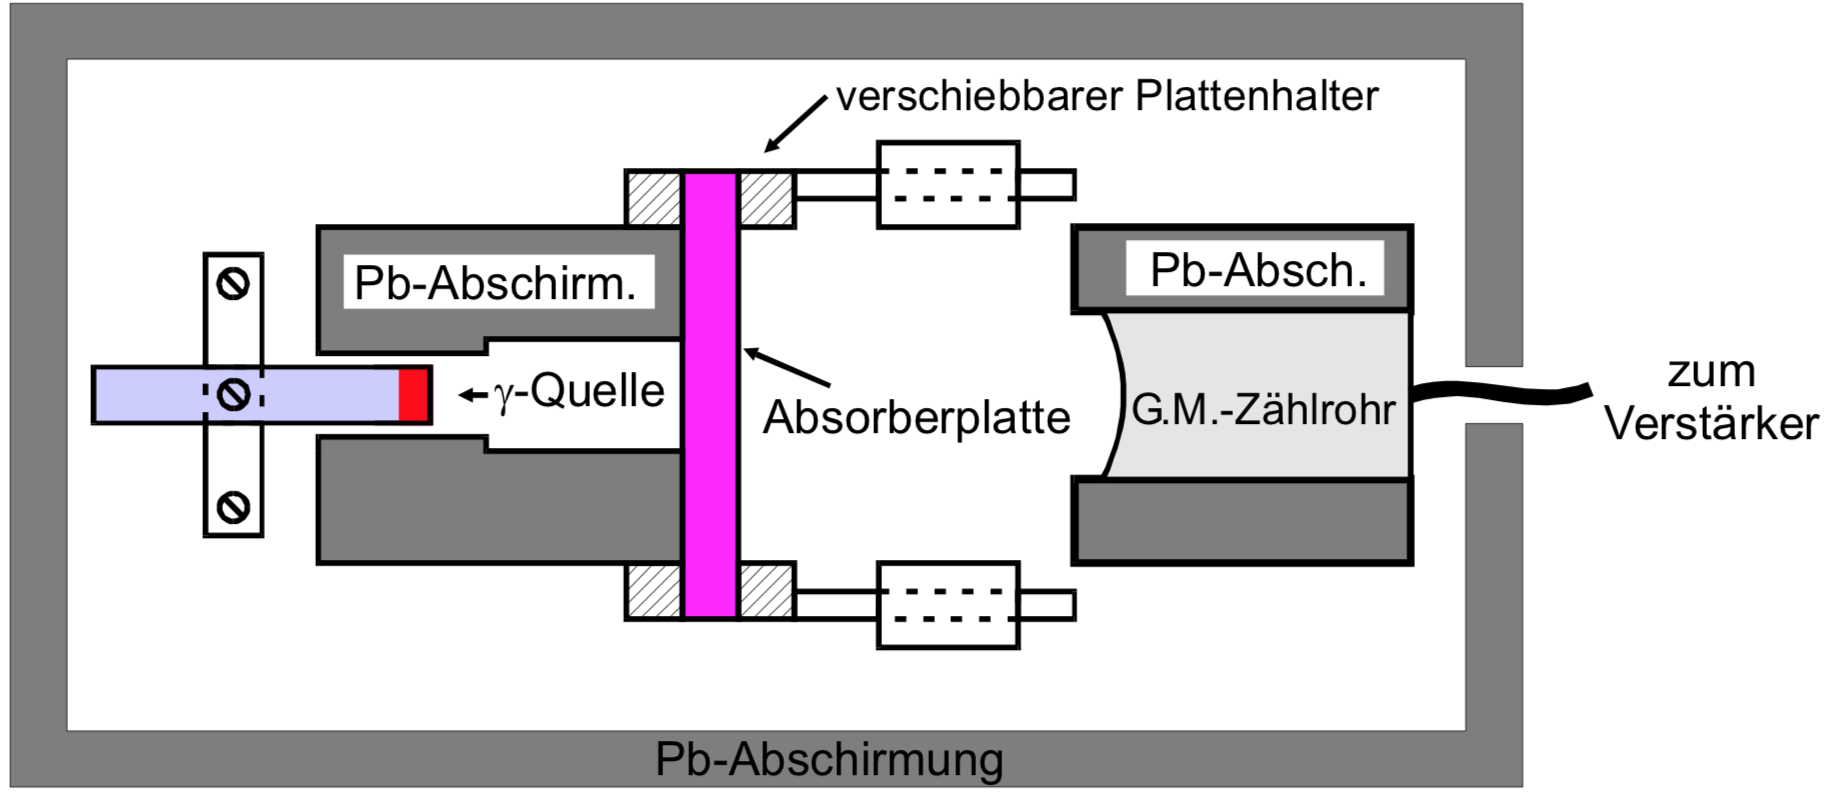
\includegraphics[height=5cm]{data/aufbau.png}
  \caption{Skizze der Messaparatur \cite{Versuchsanleitung}. Diese wird auch
  für $\beta$-Strahlung verwendet.}
  \label{fig:geraet}
\end{figure}

Daraufhin wird für $\beta$-Strahlung für Aluminiumabsorber verschiedener Dicken
die Anzahl der Impulse in einem selbst zu wählenden Zeitraum gemessen. Dabei ist
darauf zu achten, dass in jedem Zeitraum mindestens 400 Impulse gemessen werden.

Für $\gamma$-Strahlung wird für Zink- und Eisenabsorber verschiedener Dicken
die Anzahl der Impulse gemessen. Erneut ist hier auf die Wahl des Zeitraumes
zu achten.
